% !TEX root = ../notes_template.tex
\chapter{Fundamentals}\label{chp:fundamentals}
Updated on \today
\minitoc

This chapter covers fundamentals of muscle structure and function. It defines terms and explains concepts used through the book. It is expected that anyone reading this book has a background that includes Anatomy \& Physiology. Skim or even skip sections that you have already mastered. The book attempts to balance the depth and breadth of clinical physiology with a muscle centered approach for physical therapy. This means the book is not the deepest nor the broadest coverage of each topic. There are areas that you have gone deeper, but we may take a broader perspective. There are areas where you are comfortable with the breadth, but we may take a deeper perspective. Physical therapists balance depth and breadth (look down, look up and beyond) during examination, evaluation and interventions. The PT may consider the molecular effect of calcium for muscle contraction, its role within the supportive matrix of bone, its absorption and distribution through the body, and whether someone is physically capable of independently obtaining and preparing meals that provide sufficient calcium in their diet. The terms - deeper and broader - are relative.

\vspace{5mm}

\textbf{Objectives include:}
\begin{enumerate}
   \item Explain muscle \textit{in situ} .
   \item Explain muscle fidelity and efficacy. 
    \item Describe and explain the importance of the macroscopic muscle scaffold including connective tissue, tendons and bony attachments.
    \item Explain what is meant by attaining and sustaining tension.
    \item Explain the difference between active and passive tension.
    \item Describe and explain the implications of muscle pennation.
    \item Explain the contexts that result in $\Delta$ length during active tension (concentric, eccentric, isometric).
    \item Explain roles of muscles such as agonist, antagonist, synergists and stabilizers.
    \item Explain the relationship between of muscle active tension, muscle force, muscle torque and movement.
    \item Provide of an example of a free body diagram including the relevant forces to generate torques and which relationships between the torques produce different contraction types and movements.
\end{enumerate}

\section{Muscle Fibers and Muscles}
Through the book we take a muscle centered approach. Most of the time what we mean is a muscle fiber centered approach. As a clinical physiology book our emphasis is on the cellular events occurring in the muscle fiber to fulfill its act of tensioning; the fidelity, efficacy and integrity of that act; and how that act is supported by integrated physiological function. We cannot escape the reality that while muscle fibers are the basic unit of the muscle system, each muscle fiber constitutes one cell of an entire muscle. It is the muscle as a structural and functional entity that physical therapists may think about more often, whether the biceps femoris muscle is too tight or too weak, for example. We cannot lose sight of the fact that as a physical therapist you also need to be able to recognize and investigate and relate what is happening in that muscle to what is happening in its cells, and how the body is supporting those cells. The muscle includes muscle fibers and connective tissue. A single muscle fiber, alone, has a limited functional role in the moving human. It is in the collective action of muscle fibers, as a muscle, that muscle fibers play an integral functional role in the moving human. To be organized and to act as an effective collective, muscle fibers are bound together by connective tissue, and through connective tissue are attached to bones or other anatomical structures. 

\paragraph{Muscles \textit{in situ}}
The muscles that you know (biceps femoris, deltoid, gastrocnemius, extensor digitorum longus, etc) are classified and identified (named) by shape and location. Shape is determined by how the muscle fibers are connected together with connective tissue. Variations in shape occur primarily from variations in how the muscle fibers are connected together and arranged. Similar to how you can construct many different shapes with a set of similarly shaped bricks. The location of a muscle is determined by what it interacts with based on its tendon attachments. The muscles you learn in anatomy and consider as part of a physical exam when palpating and testing are muscles that are identified in their original shape and in their original location. This is the muscle \textit{in situ}.\footnotemark{}footnotetext{\textit{in situ}, adverb or adjective, meaning in original position}

The act of a muscle fiber is to create tension. Creating tension occurs in the context of the muscle fibers connected together, and in interaction with other structures through tendon connections, \textit{in situ}. Throughout the book we will center on the muscle fiber as the basic tension creating system. However, we cannot lose contact with muscle \textit{in situ} so we need to know how muscle fibers come together as muscles, and how they transmit tension to bones, and how the muscle \textit{in situ}  impacts the muscle fiber.

\section{Muscle Fidelity \& Efficacy and the Act of Tension}

The muscle fiber acts to create tension and collectively muscle fibers transmit this tension to muscles \textit{in situ}. Muscle fidelity refers to the ability of, and how well, the muscle fiber and muscle attain tension. Attain tension simply means creating tension. How much tension can be attained is often measured as force. Muscle fidelity is a quality referring to the internal capabilities and parts that allow muscle fibers and muscles to attain tension. We consider muscle fidelity at the level of the muscle fiber and at the level of the muscle. 

Muscle efficacy is a quality of how well muscle sustains and transforms tension to its intended use. Sustains tension simply means keeping a certain amount of tension in the muscle. Sustaining tension typically includes consideration of how much tension has been attained, and then integrating over time. It is measured as how long an attained amount of tension is sustained. What this means is that you must consider what has been attained in order to consider whether it can be sustained. You must attain to sustain. Muscle fibers and muscles attempt to fulfill the act of tension as efficiently as possible, and by attaining tension efficiently tension can be sustained. Efficacy is held in balance with fidelity and we can consider the efficacy of fidelity, and the fidelity of efficacy, but that need not slow us down at this point. For now, efficacy refers to how efficiently tension can be created which influences sustaining tension and this is balanced with how well tension is created, which influences attaining tension. The balance between fidelity and efficacy is notable in later chapters when we consider differentiation of muscle fibers. Some muscle fibers are optimized to attain tension at the expense of sustaining tension, and others are optimized to sustain tension at the expense of attaining tension. 

\subsection{Tension}

The act of muscle fibers and muscles is to create tension. For a definition of tension we can turn to physics: 

\begin{displayquote}
In physics, tension is described as the pulling force transmitted axially by the means of a string, a cable, chain, or similar object, or by each end of a rod, truss member, or similar three-dimensional object; tension might also be described as the action-reaction pair of forces acting at each end of said elements. Tension is the opposite of compression.\footnotemark{} \footnotetext{\url{https://en.wikipedia.org/wiki/Tension_(physics)}}
\end{displayquote}

Tension creates a pulling force between two objects. For a muscle fiber those objects are connective tissues connected to other muscle fibers serially and in parallel, or to connective tissues that connect to tendons. For a muscle those objects are bones, with tendons forming a transitional bridge between muscle fibers and bone. An important feature of the physical concept of tension is that it is related to a pulling on two objects. We can talk about pulling a rope between two objects (there is a force involved). If the objects continue to move closer to one another (to approximate each other) and the slack rope remains in place then the rope may start to compress and limit further approximation of the objects, but that is not tension, it is compression. The act of a muscle fiber is tension, not compression.\footnotemark{} \footnotetext{There may be particular muscles that compress at certain joint ranges of motion (ROM). For example, passive elbow or knee flexion can be said to have a "soft end feel" because the slackened flexion muscles are compressed which limit further flexion. A soft end feel occurs when soft tissue compression limits further ROM.}

\section{Connective Tissue Scaffold}

Building a muscle from muscle fibers requires an intricate connective tissue scaffold that connects and shapes muscle fibers. This scaffold also functions to transmit tension between muscle fibers and tendons.  This connective tissue binds muscle fibers into what we see and define as a muscle. Three connective tissue compartments connect and organize muscle fibers so that the tension created by and transmitted to the muscle fiber interacts as required with the muscle \textit{in situ}. Figure \ref{fig:muscle_scaffold.jpg} shows the hierarchical structural relationship the endomysium, perimysium and epimysium. The \textbf{endomysium} is thin layer of connective tissue that surrounds each muscle fiber. The endomysium should not be confused with the sarcolemma which is a cell membrane and also surrounds each muscle fiber. The \textbf{perimysium} is a thicker layer of connective tissue that surrounds groups of muscle fibers and forms a \textbf{fascicle}. The muscle fibers in a fascicle are arranged in parallel (and thus influences a muscle's cross sectional area (thickness). The arrangement of multiple fascicles influences both the muscle length (if fascicles are arranged in series) and pennation (if fascicles are arranged at an angle to the overall muscle's line of tension through its tendons. The \textbf{epimysium} surrounds all the fascicles to form a muscle belly (readily observed on visual observation). A muscle belly may or may not be distinguished from a muscle. This depends on context. For example, the deltoid muscle is known to have separate parts (anterior, medial and posterior), each of these parts has it's own epimysium and is thus a separate belly. The point is that the epimysium does not necessarily surround the muscle as you know it and identify it (i.e. if you identified the deltoid you'd be identifying three separate muscle bellies that are each encased in an epimysium connective tissue wrap). There are additional connective tissue wraps that do surround muscles as you know them (superficial to the epimysium), and there are additional connective tissues that surround ever more superficial layers that result in muscles being bound to one another (i.e. fascia and fascial trains), but these levels of connective tissue encasement is not covered in this book. A reminder of the fascia layer and fascial trains is easy to experience with the difference you feel between a hamstring stretch with ankle dorsiflexion vs. plantar flexion.

\begin{figure}[!ht]
    \centering
    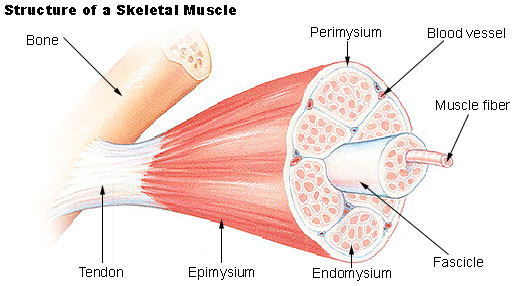
\includegraphics[width=1\linewidth]{./figure/muscle_scaffold.jpg}
    \caption{Connective Tissue Scaffold of Muscle \footnotesize{(Public Domain figure from \href{https://commons.wikimedia.org/wiki/File:Illu_muscle_structure.jpg}{Wikimedia Commons})}}
    \label{fig:muscle_scaffold}
\end{figure}

\subsection{Roles of the Connective Tissue Scaffold}

The endomysium, perimysium, epimysium connective tissue scaffold have a role in connecting, containing and arranging muscle fibers. They are also fundamental in the transmission of tension and to and through tendons to their attachments \cite{turrina_muscular_2013}; and to secure the physical location and approximation of the neurovascular supply to the muscle fibers.

\paragraph{Transmit tension}

Each muscle fiber transmits tension to one another and through the connective tissue scaffold. To transmit tension the connective tissue must securely, and with minimal elasticity, connect each muscle fiber to each other and to the tendon. The endomysium and perimysium tend to be thinner and contain both collagen and reticular fibers. Whereas the epimysium tends to have a greater volume of collagen (less elastic). 

The transmission of tension from muscle fiber to tendon to bone includes two zones of transition, muscle-to-tendon, and tendon-to-bone. The muscle-to-tendon zone is referred to as the \textbf{musculotendonous junction (MTJ)}. The MTJ is where muscle fibers start to diminish and muscle connective tissue, primarily epimysium starts to increase and meet the collagenous tendon tissue. From the muscle fibers toward the tendon the MTJ includes multi directional tendon projections gradually reorienting to being longitudinally oriented tendon tissue which allows a uniform transmission of tension. You can think of the multidirectional projections as part of the MTJ's role of integrating and summing the muscle fiber tension to be focalized in the tendon \cite{knudsen_human_2015}. Tendons consist of dense connective tissue that allows them to absorb and transmit substantial tension. Tenocytes (cells that make tendons) account for about 20\% of tendon volume, and the extracellular matrix (ECM) accounts for about 80\% of tendon volume \cite{kjaer_role_2004}. 

The tendon-to-bone zone is referred to as the tendon-bone attachment. The formation of an attachment between tendon and bone starts during embryonic development. During musculoskeletal system assembly, the tendon–bone attachment  forms a structure that is mechanically complex given the need to transfer tension between two materials that differ greatly in stiffness (tendon being non mineralized connective tissue, and bone being mineralized connective tissue).    

\paragraph{Secure the neurovascular supply}
The connective tissue scaffold secures the neurovascular supply to muscle. By secure we mean literally makes sure that the neurovascular supply stays were it is supposed to stay. By entering through epimysium and perimysium connection tissue the neurovascular structures (nerves, arteries, veins) are secure in their path regardless of what length a muscle belly may take. They are then embedded in the endomysium in close proximity to the muscle fiber with which they  interact regardless of the length of the muscle fiber. The vascular supply is delivered by arteries and arterioles, and removed by veins and venules, that provide blood flow that penetrates the epimysium and perimysium to reach the muscle fibers. Capillaries then surround each muscle fiber embedded and anchored in the endomysium to interact and exchange mass with the muscle extra-cellular fluid. Innervation of muscle for both excitation and regulation by the nervous system comes from branches of peripheral nerves that penetrate the epimysium and perimysium and terminate in and are anchored by the endomysium at the required location for each muscle fiber (at the neuromuscular end plate and further discussed in Chapter 3 on Muscle Excitation).


\section{Muscle Mechanics}

Chapter 2 on Tension focuses on the mechanisms internal to a muscle fiber for generating tension. Our inclusion of muscle fiber mechanics here is a simple first pass to serve the purpose of considering some basic topics of muscle mechanics such as passive and active tension, pennation, and the velocity of $\Delta$ length\footnotemark{}\footnotetext{$\Delta$ length refers to changes in length} during active tension.

\subsection{Active \& Passive Tension}

Tension created by a muscle fiber can be either active or passive. Active tension is generated when the muscle fiber transform chemical into mechanical energy. The mechanical energy of active tension pulls the ends of a muscle fiber together, it attempts to shorten the muscle fiber and through transmission of that tension to the connective tissue scaffold it attempts to shorten the entire muscle (bring the tendon attachments together). Passive tension is generated when another force attempts to lengthen a muscle fiber. When another muscle, or some other force attempts to pull the tendon attachments apart, which transmits tension to the muscle fibers and they lengthen without attempting to transform chemical energy into mechanical energy. 

\subsection{Pennation - Fascicle Arrangement}

Fascicle arrangement includes whether the fascicles are organized (mostly) parallel to the overall tendon line of pull, or whether there is an angle between the fascicle and the overall tendon line of pull. Figure \ref{fig:pennation} shows an arbitrary muscle with a line of pull of the whole muscle along the overall tendon line in red $F_{wm}$; and the line of pull of the muscle fibers bundled in fascicles at angle $\alpha$ in orange $F_{fiber}$. When there is an angle, such as $\alpha$, the muscle is described as being pennnated. Another way to say this is that pennation exists when there is an angle between the line of pull of the fascicles and the line of pull of the tendons.\footnotemark{}\footnotetext{Note, if the sum of all $\alpha = 0$ from one attachment to the other attachment then the muscle is not pennated. For example even in long muscles such as the biceps brachi there is, at any point along the muscle, an $\alpha$, but from one end to the other they cancel each other out because at either end they are angled in the opposite direction.} Note from Figure \ref{fig:pennation} that the line of pull of the tendons is usually the vector sum of the lines of pull of the fascicles. With pennation there is a vector component of the muscle fiber that acts in line with the tendon pull, and there is a vector component that does not work in line with the tendon pull. Typically the vectors that act in line with the tendon pull sum together; whereas the vectors that do not act in line of the tendon pull cancel each other out.\footnotemark{}\footnotetext{There are situations where the vector components not in line with the tendon line of pull do not cancel out, however in such instanes there is usually another structure that creates the forces to properly counter balance those forces}  Fascicle arrangement is - in large part - one of the primary features that distinguishes various classifications of muscles; and the unique fascicle arrangement, along with shape, even within a classification can help distinguish particular muscles from one another.


\begin{figure}[!ht]
    \centering
    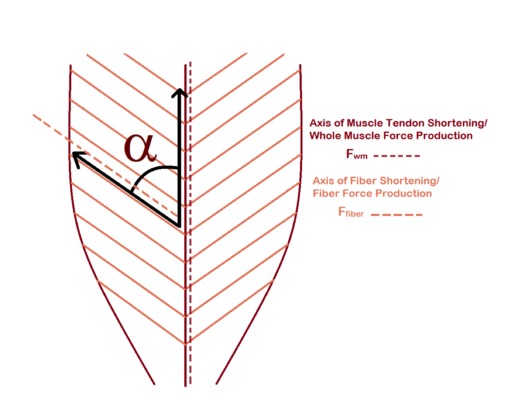
\includegraphics[width=1\linewidth]{./figure/pennation.png}
    \caption{Pennation of Muscle Fibers \footnotesize{(Public Domain figure from \href{https://commons.wikimedia.org/wiki/File:Pennation_angle_of_fibers_in_pennate_muscle.png}{Wikimedia Commons})}}
    \label{fig:pennation}
\end{figure}

Fascicle arrangement is a muscle \textit{in situ} factor that influences the velocity of shortening of the muscle per unit of shortening of a muscle fiber; and the muscle force produced, per unit of force of a muscle fiber. Overall it is not a modifiable aspect of a muscle, meaning there are no training (stretching, pulling, needling, strengthening) programs that alter a particular muscles pennation status (whether it is pennated or not). Though there is evidence of training influencing, in small degrees, the angle of pennation \cite{cuthbert_effect_2020}.

\paragraph{Velocity of Shortening}
 
If two muscles, one pennated and one not pennated, had a set of homogeneous muscle fibers that all shortened at the same velocity during active tension with no resistance. The muscle without pennation would shorten with a higher velocity. This occurs because the shortening of each fiber is summed to the whole muscle. If each fiber shortens to 50\% of its length in one second, then the muscle as a whole would shorten to 50\% of its length in one second. However, in a pennated muscle, when each fiber shortens to 50\% of its length in one second, the muscle as a whole shortens at about 50\% $\times \cos(\alpha)$ (recall that $\alpha =$ angle of pennation). For example, if $\alpha = 35^\circ$ then with all muscle fibers shortening 50\% in 1 second there would be about 40\% in 1 second.

\paragraph{Force of Active Tension}

For reasons you may already know, and that we will cover in Chapter 2 on Tension, the amount of force that a muscle can develop during maximal active tensioning is proportional to the cross sectional area of the muscle. The force of the whole muscle is proportional to the number of parallel muscle fibers that are actively generating tension. Note the stipulation that these fibers must be parallel. Adding muscle fibers in series (which make a muscle longer but not thicker) do not contribute to the force generated by the entire muscle (at its ends) because each muscle fiber, indeed each of many elemental units within the muscle fiber, pull from both ends when generating active tension and thus some of the force that they generate, in series, is cancelled out. In Figure \ref{fig:Sacromeres_series_parrallel} there are three fibers in series (A) and in parallel (B). When in series the forces from 1 and 2 cancel each other out and the force of 3 is transmitted to the the ends. When in parallel the forces of the three sum. Note that the muscle fibers in parallel increase the cross sectional area.

\begin{figure}[!ht]
    \centering
    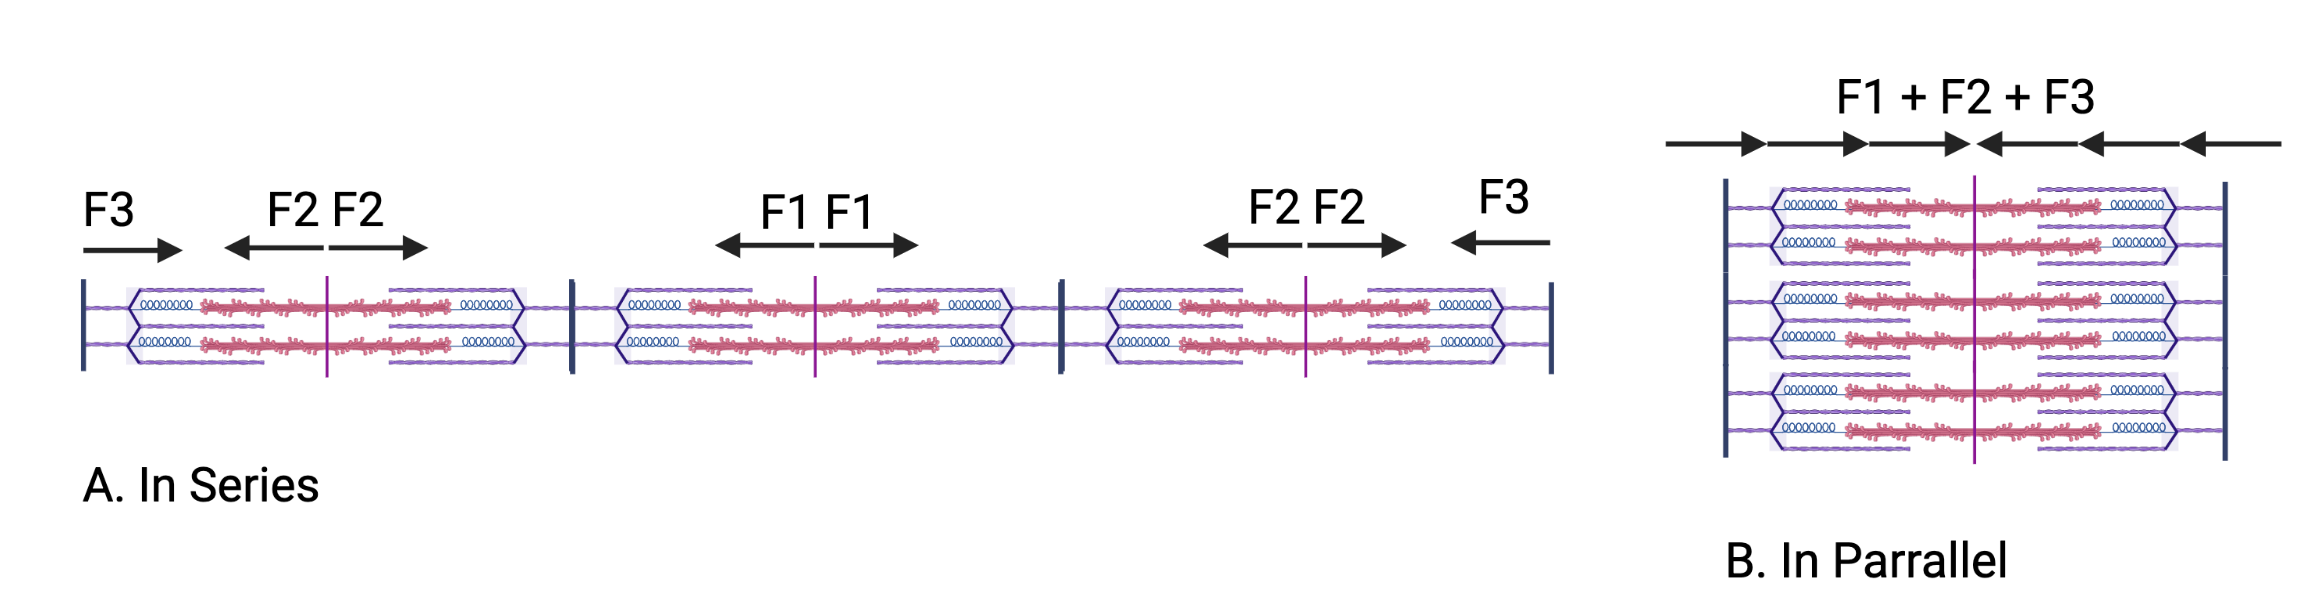
\includegraphics[width=1\linewidth]{./figure/Sarcomeres_series_parrallel.png}
    \caption{Muscle Fibers in Series \& Parallel \footnotesize{(Created with Biorender.com}}
    \label{fig:Sacromeres_series_parrallel}
\end{figure}


Pennation tends to increase the cross sectional area (the number of muscle fibers in parallel). The increase in cross sectional area is enough to compensate for any loss in force associated with the vector sum. Similar to the loss of velocity in a pennated muscles, not all of the muscle fiber tension is transmitted to the line of pull of the tendon and thus is lost. But, given the additional fibers in parallel it makes up for the loss due to the vector sum. For example, if a muscle fiber can generate 1 unit of force and we have 50 fibers in parallel the muscle as a whole can generate 50 units of force. If we can get 100 fibers in parallel with a pennated arrangement of those fibers with an angle of pull that transmits 70\% of the force to the line of pull of the tendon then the muscle can generate 70 units of force. So, despite a slight loss of efficacy at the level of the muscle fiber (less tension transmits to the line of pull of the tendon), there is a gain in fidelity at the level of the muscle (generates more tension). Whereas muscles that are not pennated (fusiform or strap muscles) tend to have higher velocities of shortening during unresisted active tension and lower maximal forces during resisted active tension.

\paragraph{Overall Effect of Pennation}
The overall effect of pennation tends to be a decrease in velocity of shortening during unresisted active tension and an increase in maximal force during resisted active tension. Keep in mind that these are these are not variations that occur due to muscle adaptations to training or other modalities (pennation or not pennation). There is some evidence that angles of pennation can be modified slightly, and there is certainly evidence that all muscles can change their cross sectional area regardless of their pennation status. As you learn the anatomy of various muscles in your physical therapy education you should consider what that muscle tends to be used for and how whether that muscle is, and if so, how it is, pennated. It is also important to consider how muscles tend to work together in groups and how groups of muscles tend to complement one another in their synergistic roles.

\subsection{$\Delta$ Length During Active Tension}

Let’s consider $\Delta$ length a change in length of a muscle, \footnotemark{}\footnotetext{For now we will not consider whether there is a change in muscle fiber length or the dynamics that are occurring within the muscle fiber.} and that negative $\Delta$ length indicates a muscle shortens, positive $\Delta$ length indicates a muscle is lengthening and zero $\Delta$ length occurs when a muscle does not change length. We can now name various “contraction” types (as they are commonly known) based on the $\Delta$ length during active tension. 

\begin{table}[h!]
\centering
\begin{tabular}{||c c c ||} 
 \hline
 $\Delta$ Length & Muscle & Contraction Type \\ [0.5ex] 
 \hline\hline
 Negative & Shortens & Concentric \\
 Zero & Does not change & Isometric \\[1ex] 
 Positive & Lengthens & Eccentric \\[1ex] 
 \hline
\end{tabular}
\caption{Classification of $\Delta$ Length During Active Tension}
\label{table:contraction_types}
\end{table}


An important consideration to the concept known as contraction types is that anything other than a concentric contraction includes other counteracting forces. A muscle outside of its connected interaction space (not \textit{in situ}) will shorten (negative $\Delta$ length) with active tension.\footnotemark{} \footnotetext{Note that we are here assuming a full tetanic sequence of excitation contraction coupling as will be covered in upcoming chapters.} Therefore, the contingencies of 0 $\Delta$ length or positive $\Delta$ length are dependent on what is occurring in the system which includes all of the other interactions by other muscles and other external forces acting on the joint(s) that the muscle we are considering on it acting. And since the forces acting on joints create joint movement based on the torque being created, we can say that whether a muscle has a concentric, isometric or eccentric contraction depends on the balance between torque it is creating and the torque being created by all other forces acting at the joint.

\subsubsection{Example of how torque influences muscle contractions during active tension}

Figure \ref{fig:free_body_diagram} is a free body diagram (a simplified model) of the forces and related torque during the nordic hamstring exercise (NHE). During this exercise the subject is on their knees with their ankles supported so that the lower limb (below the knee) cannot move. The subject keeps their hips straight and slowly shifts their body mass forward. Once the body mass (black arrow) is anterior to the axis of rotation of the knee it creates a knee extension torque (black circular arrow). The subject allows themselves to not fall forward to quickly but usually reaches a point where they can no longer slow their descent and they fall to the floor. While they are attempting to slow their descent to the floor they are using their hamstring muscles which create a force through active tension (red arrow), which then creates a knee flexion torque (red circular arrow). The exercise can be done a variety of ways. In one scenario the subject can stop and hold themselves in one position. In another scenario, after holding themselves they can use the force of hamstring active tension to bring them upright again. 

\begin{figure}[!ht]
    \centering
    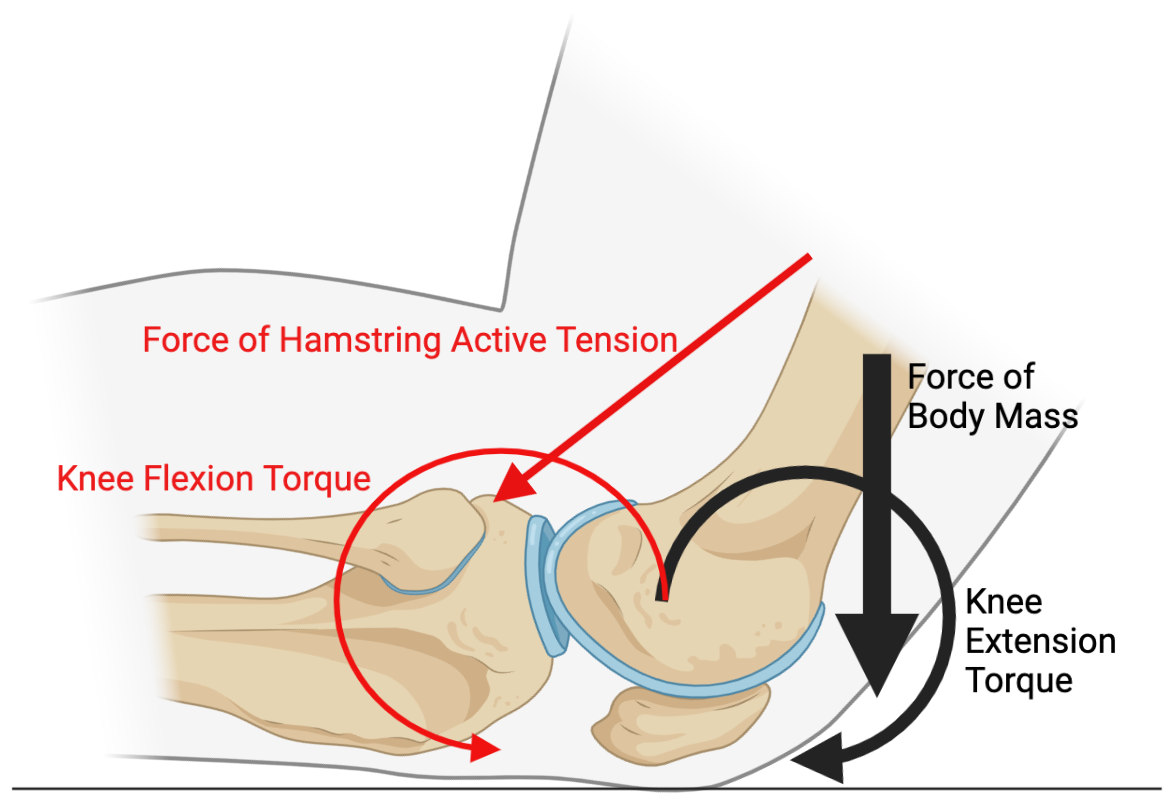
\includegraphics[width=1\linewidth]{./figure/free_body_diagram.png}
    \caption{Free Body Diagram of the Nordic Hamstring Exercise \footnotesize{(Created with Biorender.com}}
    \label{fig:free_body_diagram}
\end{figure}

There is a relationship between the force of the body mass ($F_{bm}$) and the extension torque created by the body mass ($T_{bm}$), just as there is a relationship between the force of the muscle ($F_{m}$) and the flexion torque created by the muscle ($T_{m}$). The force varies based on how much tension is created. The movement varies based on the relationship between the two opposing torques as seen in Table \ref{table:NHE}. It is important to note that the movement and the contraction types are dependent on the relationship of the torques, and the torques are related to both the force generated by the tension of the muscle, the body weight and their respective perpendicular distances.\footnotemark{}\footnotetext{This book will not spend much time at this level of analysis. However, if you are not comfortable with torque and vectors from physics and other courses you have had it is a worthwhile to refresh your memory now.}

\begin{table}[h!]
\centering
\begin{tabular}{||c c c c c||} 
 \hline
 Torque Relationship & $\Delta$ Length & Muscle & Contraction Type & Movement\\ [0.5ex] 
 \hline\hline
$T_m > T_{bm}$ & Negative & Shortens & Concentric & Knee Flexion \\
$T_m = T_{bm}$ & Zero & Does not change & Isometric & No Movement\\[1ex] 
$T_m < T_{bm}$ & Positive & Lengthens & Eccentric & Knee Extension \\[1ex] 
 \hline
\end{tabular}
\caption{$\Delta$ Length During Active Tension Based on Torque Relationships}
\label{table:NHE}
\end{table}

\section{Muscle Roles}

\begin{itemize}
\item Agonist: Muscle creating tension for the intention of the movement.
\item Antagonist: Muscle that creates the opposite movement of the agonist.
\item Synergists: Muscles that work together and combine their tension to create a movement. We can talk about synergist agonists and synergist antagonists, though the former is typically the intention when just referring to synergists.
\item Stabilizer: Muscles that provide tension to neutralize certain motions toward the purpose of a movement
\end{itemize}

To define a muscle role we must consider context. Context for muscle roles are typically movements. Movements include all the motions that are occurring, the directions of those motions and the intention of the mover doing the movement. For example, if the movement is the downward phase of a squat one of the motions is knee flexion. The intention of the mover is knee flexion (they intend to move downward). The knee extensor muscles are involved as agonists even though knee is flexing. Just because the motion is knee flexion, the agonists are not the knee flexors.



\section{Summary \& Next Step}

This chapter covered some of the fundamentals of muscle function such as fidelity and efficacy and how they related to attaining and sustaining tension. We discussed how the connective tissue scaffold allows muscle fiber tension to transmit to the muscle tendon and bony attachments for the purpose of whole muscle tension, including what it means to consider a muscle \textit{in situ}, and how that same scaffold provides an anchor for the neuromuscular supply and the overall shape of a muscle, including fascicle arrangement. Fascicle arrangement influences how the muscle \textit{in situ} force and length is related to muscle fiber force and $\Delta$ length. And how not only a particular muscle’s active tension, but other forces, have an integral influence the $\Delta$ length of a muscle during active tension and therefore contraction type. Finally we classified four muscle roles, agonist, antagonist, synergist and stabilizer. The next chapter covers the muscle fiber and considers its structure and the mechanisms involved in attaining and sustaining both active and passive tension.

\printbibliography[heading=subbibintoc]


